\chapter{Introduction}
\section{Background}
Power electronic converters are an electrical circuit that convert electrical energy
from on level of voltage/current/frequency to another using a semiconductor based 
electronic switches and energy storage components \cite{holmes2003pulse,mohan2003power,
rodriguez2012predictive}. As the demand for expansion of renewable energy and high efficiency
energy conversion is growing, power electronic systems are widely being used to process
the available power to meet load requirements. For this reason, a Three-Phase AC/DC active
rectifier has been gaining momentum in high power electric vehicles (EV) charging stations,
renewable energy generation, industrial motor control and power supplies.\par

Traditionally, rectifiers based on diodes and thyristors are able to provide uncontrolled
and controlled DC Output respectively. But both converters have low power factor, 
non-sinusoidal input current, high input harmonic distortion and low-frequency voltage 
ripple in the output side which requirements large filters in both AC and DC sides, However
those filters are very costly and bulky. With the development self-commutating power electronic
devices (MOSFET, IGBT \& GTO etc.) many topologies have developed to overcome the shortcomings 
of the conventional converters, such as multilevel, multipulse, boost, buck, PFC etc.
\cite{articleKolarI,articleKolarII,ReviewSafayatullah,batteries9030150}. Among the
improved power converters, a Pulse Width Modulation (PWM) based power converters preferred for 
their high efficiency.\par

The three phase two level boost rectifier shown in fig.\ref{fig:topology} is a PWM controlled,
low-cost, well-known and robust topology consisting of six active switches, a DC link capacitor and 
three AC side inductors with continuous input current, bidirectional power flow capability and 
nearly unity power factor performance. Since the output of the rectifier is connected to DC 
capacitor, which often supplies a controlled DC voltage, it is called a \textit{voltage source rectifier} (VCR).
\begin{figure}[ht]
    \centering
    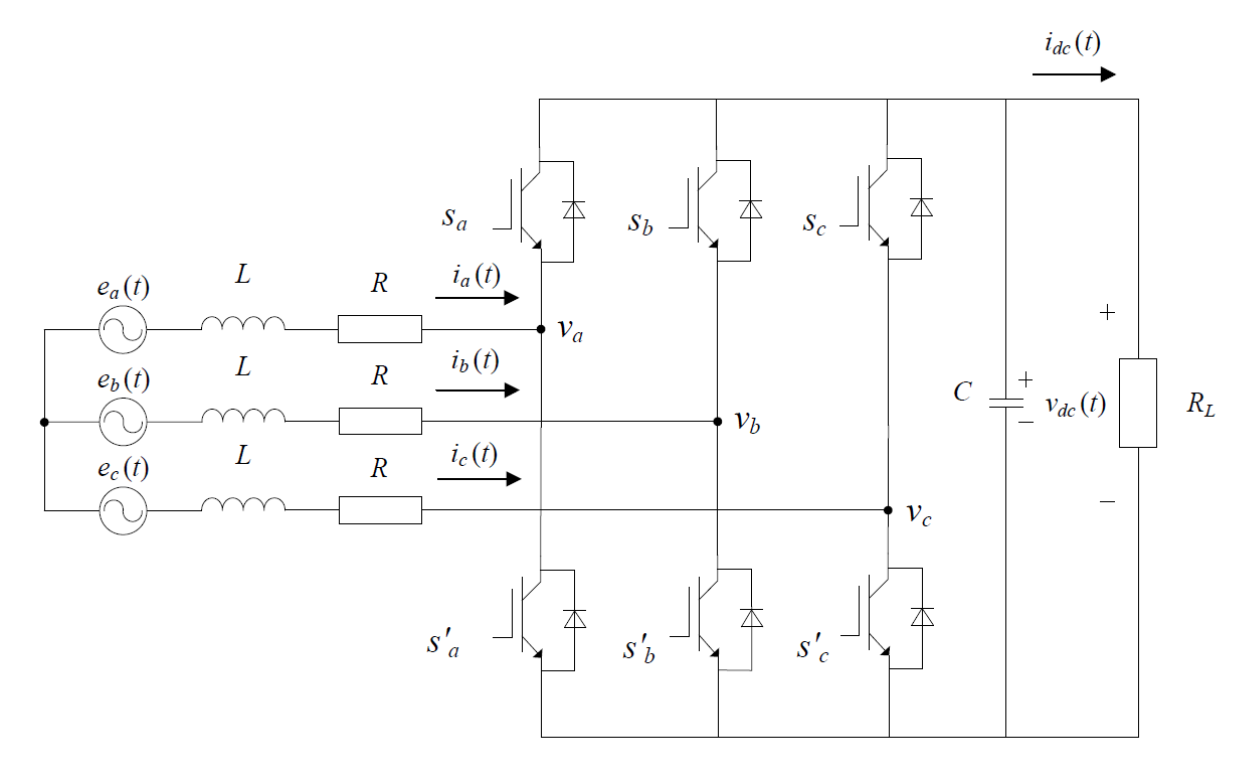
\includegraphics[scale=0.4]{img/twolevelvsctopology.PNG}
    \caption{Basic topology of three phase two level VSR}
    \label{fig:topology}
\end{figure}
\section{Literature review}
\section{Statement of the problem}
\section{Objective}
\begin{itemize}
    \item Develop a mathematical model for the three phase PWM AC-DC voltage source
    rectifier in positive and negative sequence under the distorted and unbalanced operating conditions
    \item Develop a discretized Prediction Model from the mathematical model
    \item Selection of cost function and weighting factor design
    \item Design of cost function minimization
    \item Simulation of the controller and VSR under different test conditions
\end{itemize}
\section{Thesis organization}